\begin{frame}
\frametitle{Поток исполнения}
\begin{itemize}
    \item<1->Поток исполнения - это код и его состояние (a. k. a. контекст)
    \begin{itemize}
       \item<2->код - набор инструкций в памяти, на который
       указывает регистр \emph{RIP};
       \item<3->контекст потока включает значения регистров и память.
    \end{itemize}
\end{itemize}
\end{frame}

\begin{frame}
\frametitle{Потоки и процессы}
\begin{itemize}
    \item<1->Поток работает в контексте некоторого процесса
    \begin{itemize}
        \item<2->т. е. поток "живет" в логическом адресном пространстве процесса;
        \item<3->несколько потоков могут работать в рамках одного процесса;
        \item<4->процесс имеет как минимум один поток.
    \end{itemize}
\end{itemize}
\end{frame}

\begin{frame}
\frametitle{Стек потока}
\begin{itemize}
    \item<1->Каждый поток исполнения имеет свой собственный стек
    \begin{itemize}
        \item<2->стек хранит адреса возвратов и локальные переменные;
        \item<3->для процессора стек - место в памяти, куда указывает
        \emph{RSP}.
    \end{itemize}
\end{itemize}
\end{frame}

\begin{frame}
\frametitle{Многопоточность}
\begin{itemize}
    \item<1->В системе могут \emph{одновременно} работать несколько
    потоков исполнения
    \begin{itemize}
        \item<2->на нескольких ядрах процессора;
        \item<3->на одном ядре, создавая \emph{иллюзию} одновременной работы.
    \end{itemize}
\end{itemize}
\end{frame}

\begin{frame}
\frametitle{Многопоточность}
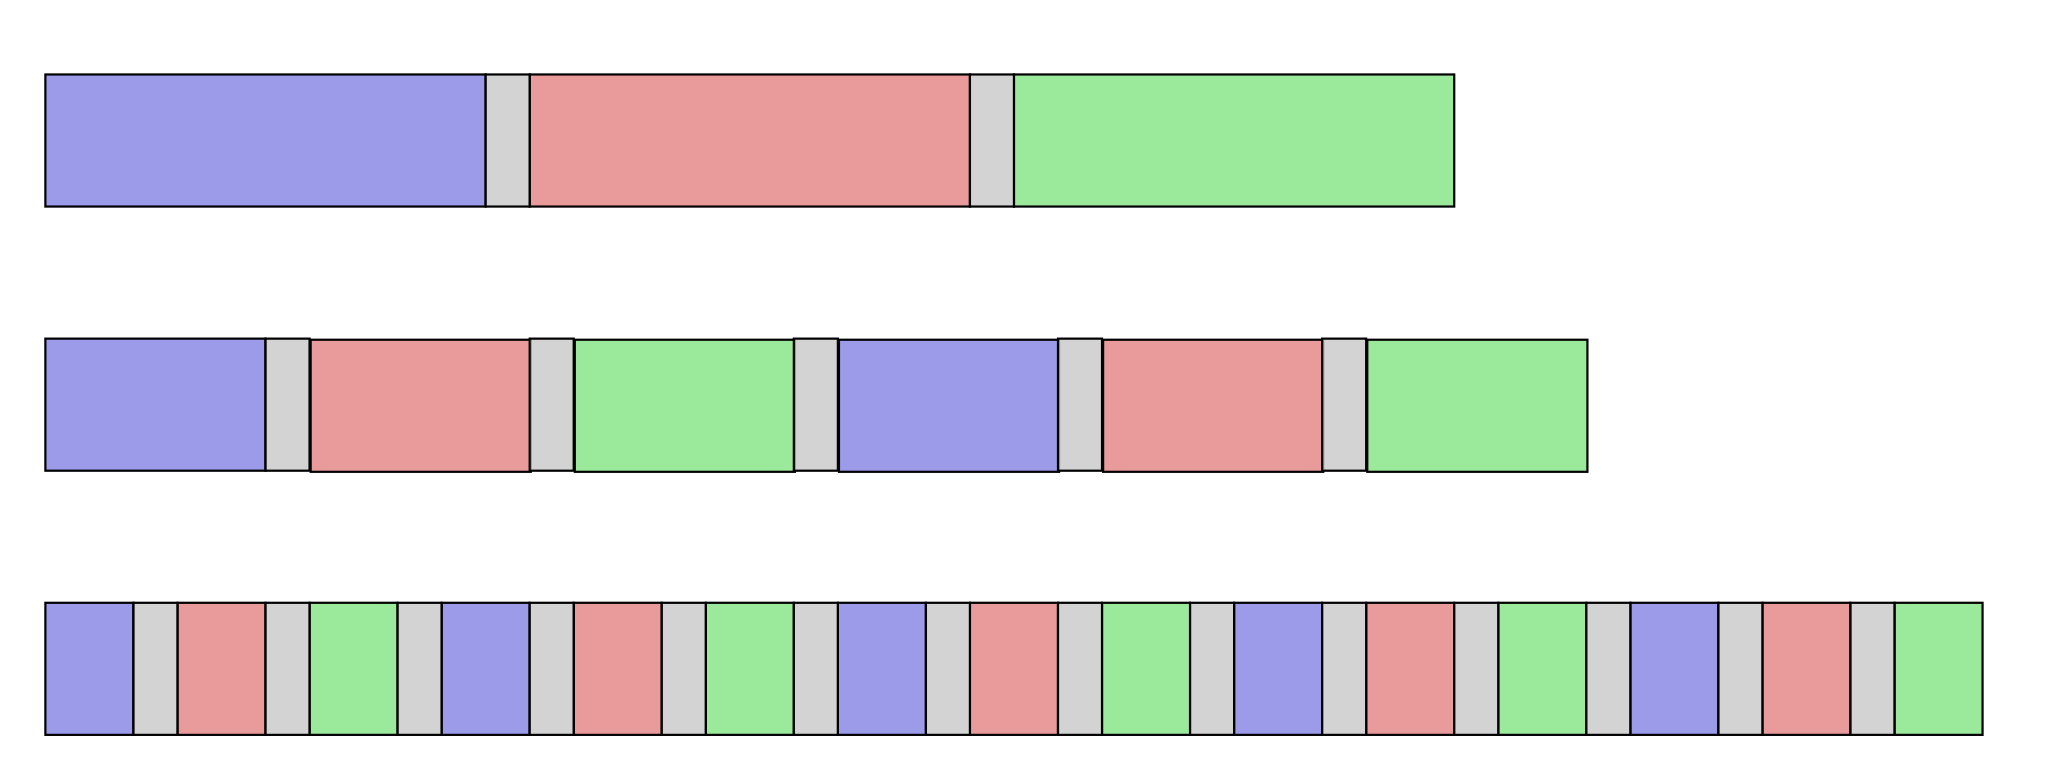
\includegraphics[height=.3\textheight]{multithreading}
\end{frame}

\begin{frame}
\frametitle{Переключение между потоками}
\begin{itemize}
    \item<1->Для переключения между потоками необходимо:
    \begin{itemize}
        \item<2->сохранить контекст исполняемого потока;
        \item<3->восстановить контекст потока, на который мы переключаемся.
    \end{itemize}
\end{itemize}
\end{frame}

\begin{frame}[fragile]
\frametitle{Пример переключения для x86}
\begin{lstlisting}
    .text
switch_threads:
    pushq %rbx
    pushq %rbp
    pushq %r12
    pushq %r13
    pushq %r14
    pushq %r15
    pushfq

    movq %rsp, (%rdi)
    movq %rsi, %rsp

    popfq
    popq %r15
    popq %r14
    popq %r13
    popq %r12
    popq %rbp
    popq %rbx

    retq
\end{lstlisting}
\end{frame}

\begin{frame}[fragile]
\frametitle{C API}
\begin{itemize}
    \item \lstinline|void switch_threads(void **prev, void *next);|
    \item<1->по завершении функции \lstinline|*prev| будет указывать
             на сохраненный контекст;
    \item<2->\emph{next} указывает на сохраненный контекст потока, на
             который мы переключаемся.
\end{itemize}
\end{frame}

\begin{frame}[fragile]
\frametitle{switch\_threads}
\begin{lstlisting}
    .text
switch_threads:
    /* save contex on stack */
    pushq %rbx
    pushq %rbp
    pushq %r12
    pushq %r13
    pushq %r14
    pushq %r15
    pushfq

    /* rdi - the first argument */
    movq %rsp, (%rdi)

    /* rsi - the second argument */
    movq %rsi, %rsp

    /* restore from stack */
    popfq
    popq %r15
    popq %r14
    popq %r13
    popq %r12
    popq %rbp
    popq %rbx

    retq /* ! */
\end{lstlisting}
\end{frame}

\begin{frame}
\frametitle{Переключение потоков}
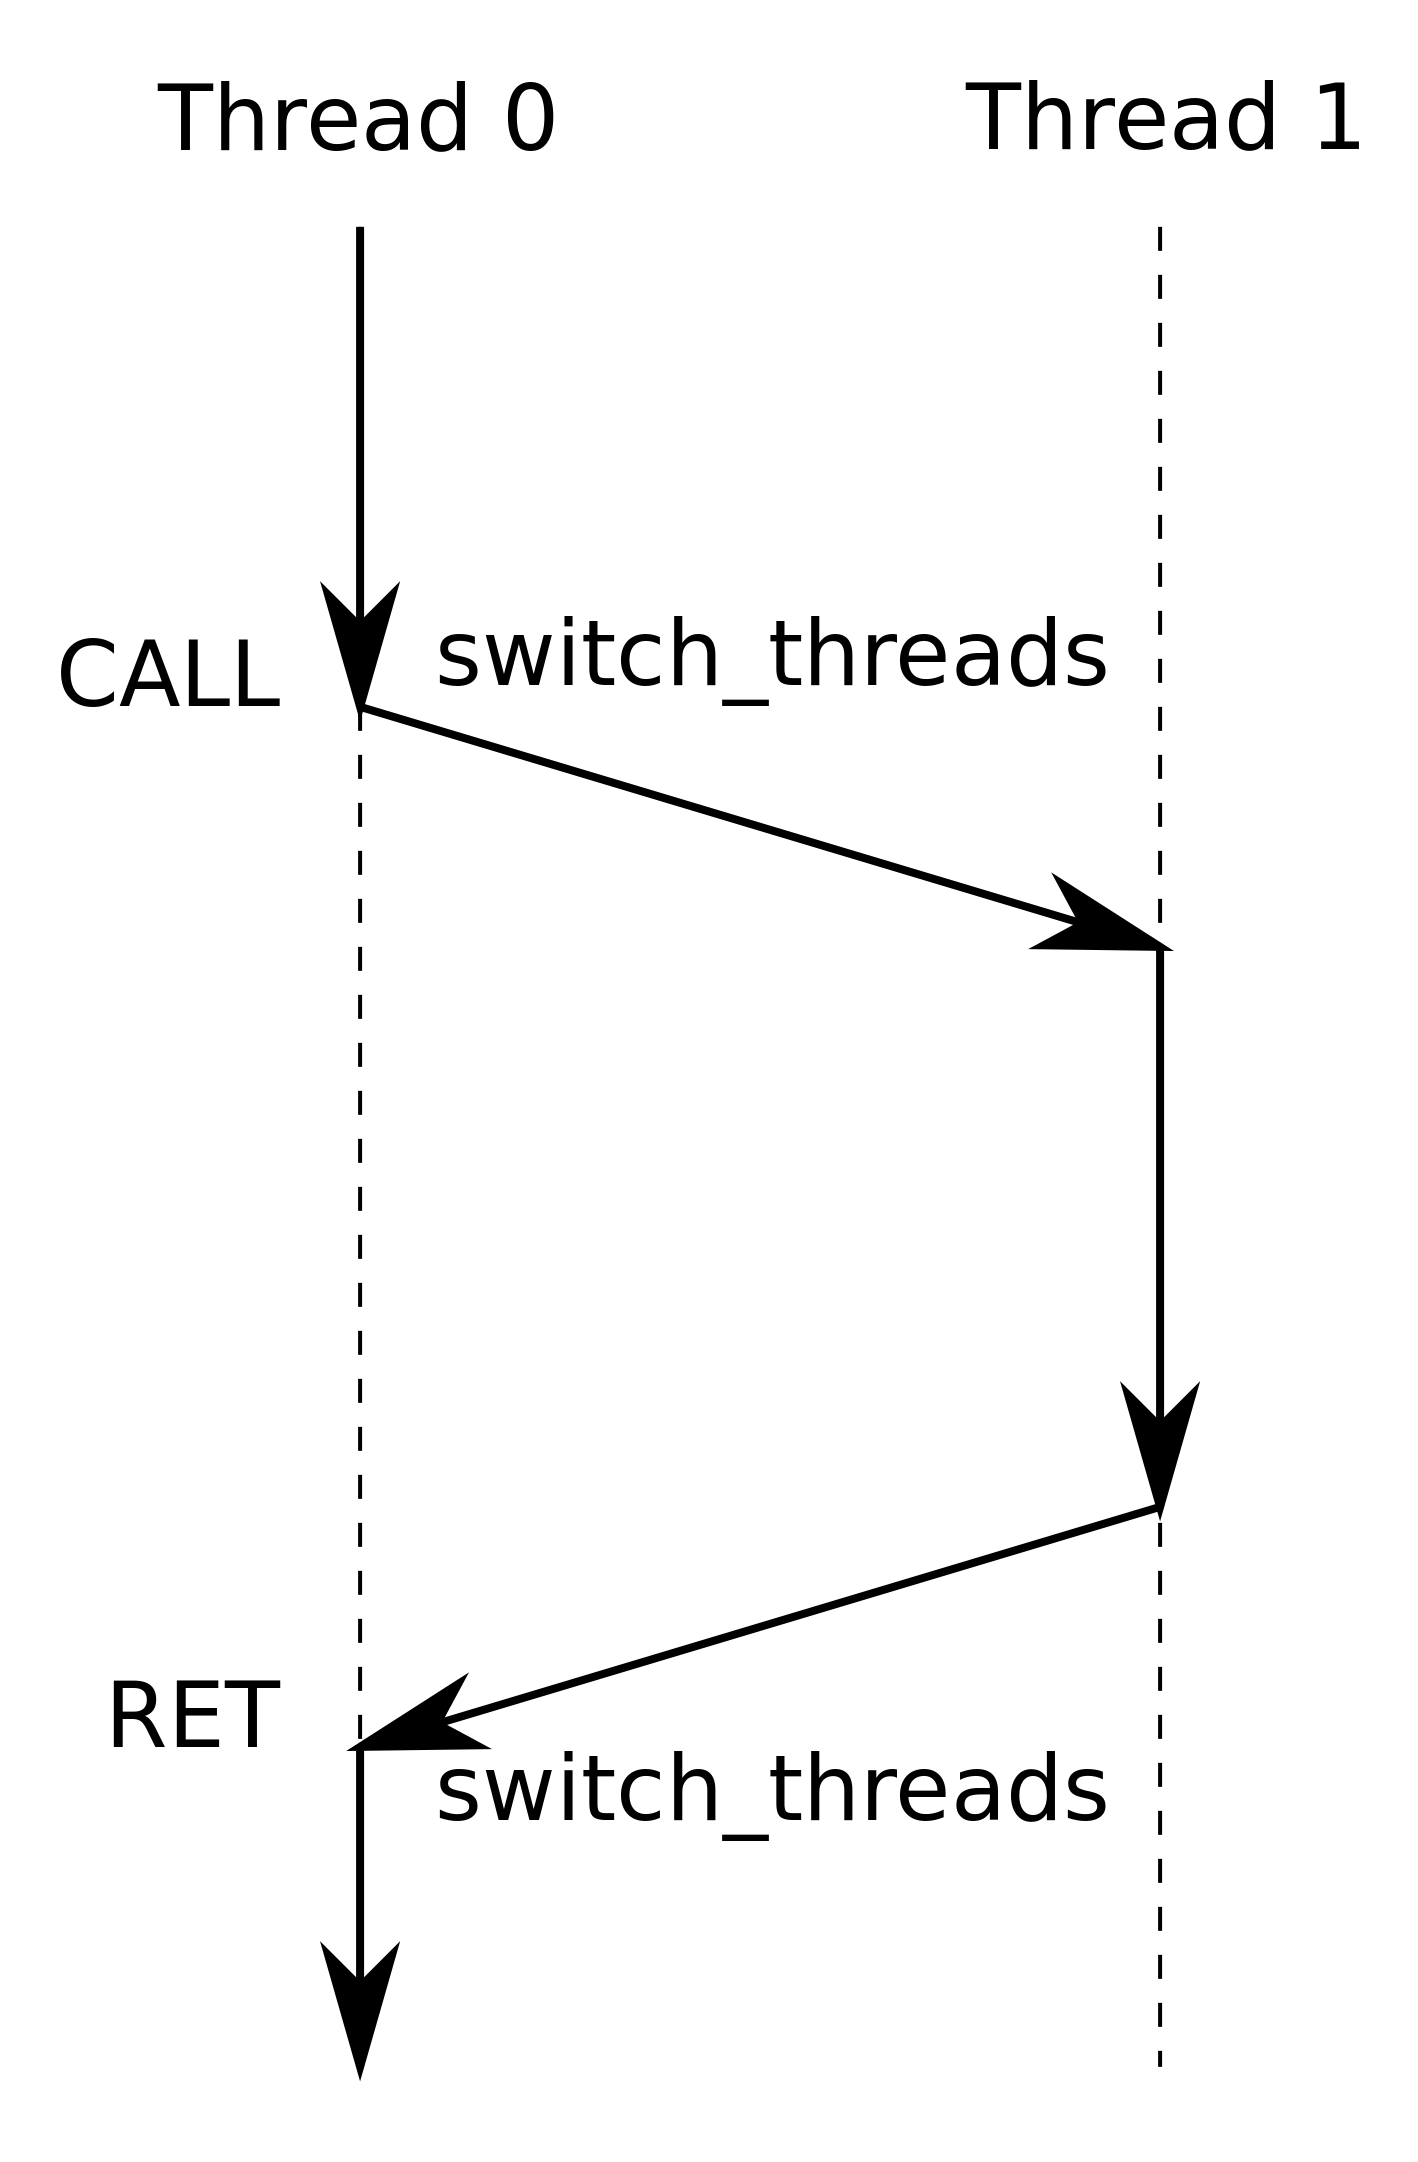
\includegraphics[height=.8\textheight]{switch}
\end{frame}

\begin{frame}
\frametitle{Создание нового потока}
\begin{itemize}
    \item Как создать новый поток и переключиться на него в первый раз?
    \begin{itemize}
        \item<1->нам нужно выделить место для хранения указателя на контекст;
        \item<2->нам нужно выделить место под стек нового потока;
        \item<3->нам нужно сохранить на стеке начальный контекст и сохранить
        указатель на него.
    \end{itemize}
\end{itemize}
\end{frame}

\begin{frame}[fragile]
\frametitle{Начальный контекст}
\begin{lstlisting}
struct switch_frame {
    uint64_t rflags;
    uint64_t r15;
    uint64_t r14;
    uint64_t r13;
    uint64_t r12;
    uint64_t rbp;
    uint64_t rbx;
    uint64_t rip;
} __attribute__((packed));
\end{lstlisting}
\end{frame}
